\section{Durchführung}
\label{sec:Durchführung}

In diesem Teil wird das Zählrohr von einer $\beta$-Strahlenquelle mit
$\beta$-Teilchen beschossen. Die daraus entstehende Zählrohrstrom wird dann von
einem Strommessgerät gemessen und die entstehende
Spannungsunterschiede werden über einen Kondensator zu einem Verstärker
"weitergeleitet", wo diese dann gezählt werden, dies ist in der
Abb. \ref{fig:VA} dargestellt.
Wird nun die Spannung varriiert kann die Abhängigkeit der Zählrate von der Spannung
untersucht werden. Außerdem wird versucht, die Nachentladungen an einem Oszilloskop
sichtbar zu machen. Mit dem Oszilloskop wird auch die Totzeit abgeschätzt, indem
grob abgelesen wird, wie lang die Abklingzeit der Impulse ist.

Um die Totzeit genauer zu bestimmen wird  eine zweite Quelle hinzugezogen und
nach der Zweiquellenmethode gemäß \eqref{eqn:2Quellen}, bzw \eqref{eqn:easy}
vorgegangen.

\begin{figure}
  \centering
  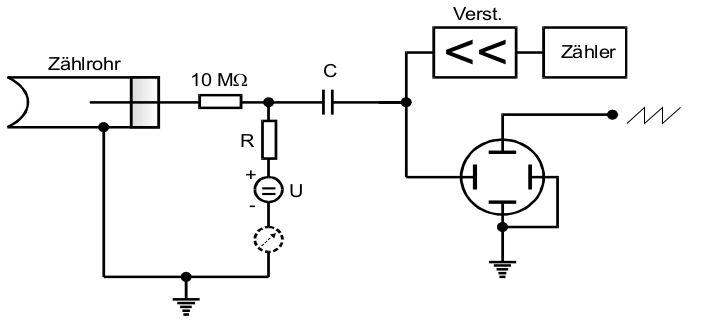
\includegraphics[height=5cm]{logos/Aufbau.png}
  \caption{Schematischer Versuchsaufbau}
  \label{fig:VA}
\end{figure}
